%!TEX root = ../dokumentation.tex

\section{Installationsschritte}

Die Projekte für „Client“ und „Server“ liegen jeweils als Eclipse Projekt vor.\\

\paragraph{Client - Entwicklungsumgebung}

\begin{enumerate}
	\item Für die Entwicklungsumgebung der „Client“ Anwendung muss zunächst Eclipse IDE for Java Developers\footnote{\url{http://www.eclipse.org/downloads/moreinfo/java.php}, zuletzt gesichtet am 13. Januar 2014} installiert werden.
	\item Das aktuelle Software Development Kit\footnote{\url{http://developer.android.com/sdk/index.html\#ExistingIDE (Menü aufklappen)}, zuletzt gesichtet am 13. Januar 2014} muss geladen und entpackt werden
	\item Anschließend muss das „Android Development Tools“ Plugin\footnote{\url{http://developer.android.com/sdk/installing/installing-adt.html}, zuletzt gesichtet am 13. Januar 2014} für Eclipse heruntergeladen und installiert werden.
	\item Der im Plugin enthaltene SDK Manager muss dann so konfiguriert werden, dass er den Pfad zu dem bereits heruntergeladen SDK kennt.
	\item Nach der Konfigration müssen weitere Tools und Pakete geladen werden, siehe Abb. \ref{fg:android-sdk-manager}.
	\begin{figure}[H]
		\centering
		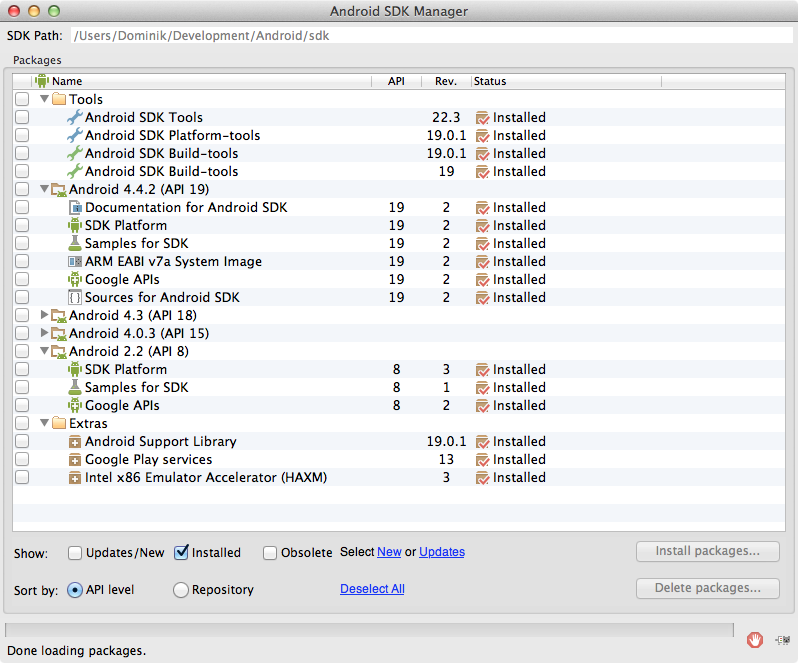
\includegraphics[width=0.85\textwidth]{./images/install/android-sdk-manager.png}
		\caption{SDK Manager: Pakete, die installiert werden müssen.}
		\label{fg:android-sdk-manager}
	\end{figure}
	\item Optional: Falls kein Testgerät vorliegt, welches den Anforderungen entspricht, kann ein „Android Virtual Device“ (AVD)\footnote{\url{http://developer.android.com/tools/devices/index.html}, zuletzt gesichtet am 13. Januar 2014} eingerichtet werden. In unseren Tests hat sich ein AVD auf Basis des Nexus One (Abb. \ref{fg:android-adv}) als hilfreich erwiesen. Wichtig ist, dass bei \textit{Target} ein Wert mit \textit{Google APIs} als Präfix ausgewählt wird.
	\begin{figure}[H]
		\centering
		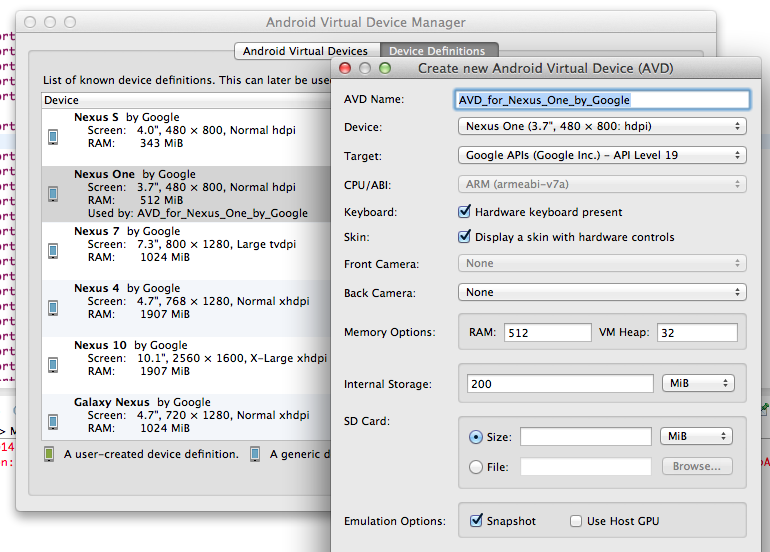
\includegraphics[width=0.85\textwidth]{./images/install/android-avd.png}
		\caption{AVD auf Basis des Nexus One}
		\label{fg:android-adv}
	\end{figure}
	\item Die Applikation kann über das Kontextmenü des Projektes unter \textit{Run As -> Android Application} ausgeführt werden.
\end{enumerate}


\paragraph{Client - Device}

\begin{enumerate}
	\item Nachdem das Projekt einmal als Android-Anwendung im Emulator oder auf dem Testgerät ausgeführt wurde, befindet sich im \texttt{bin} Verzeichnis des Projekts die Datei \texttt{FindYourCamp.apk}. Diese kann kopiert werden und beispielsweise über Dropbox auf das Gerät kopiert werden
	\item Die APK kann dann auf dem Endgerät installiert werden. Zunächst muss dazu, falls nicht schon aktiviert, die Funktion zur manuellen Installation aktiviert werden. Dazu im Menu Einstellungen unter den Punkt \textit{Sicherheit} den Haken hinter \textit{Unbekannte Herkunft} setzen.
	\item Hinweis: Der Server muss für die vollständige Funktionalität laufen.
\end{enumerate}

\paragraph{Server}

\begin{enumerate}
	\item Die Serveranwendung benötigt einen MySQL Instanz. Die Installationsanweisung für ihre Systemungebung entnehmen Sie bitte dem offiziellen Handbuch: \url{http://dev.mysql.com/doc/refman/5.1/de/installing.html}
	\item Die Zugangsdaten sowie der Datenbankname ist in der Datei \texttt{DbConfig.java} im Paket \texttt{de.fhkoeln.gm.findyourcamp.server.db} zu hinterlegen.
	\item Für die Serveranwendung muss nun die \texttt{Main.java} im \texttt{de.fhkoeln.gm.findyourcamp.server} Paket als Java-Anwendung ausgeführt werden.
	\item Hinweis: Die Anwendung ist ohne GUI konzipiert. Die Ausgabe wird über die Konsole gesteuert.
\end{enumerate}
